\ifdefined\included
\else
\documentclass[a4paper,11pt,twoside]{StyleThese}
\usepackage{amsmath,amssymb, amsthm}             % AMS Math
\usepackage[T1]{fontenc}
\usepackage[utf8x]{inputenc}
\usepackage{babel}
\usepackage{datetime}

\usepackage{silence}

\WarningFilter{minitoc(hints)}{W0023}
\WarningFilter{minitoc(hints)}{W0028}
\WarningFilter{minitoc(hints)}{W0030}

\usepackage{lmodern}
\usepackage{tabularx}
%\usepackage{tabular}
\usepackage{multirow}
\usepackage{xspace}

\usepackage{subfig}
\usepackage[inline]{enumitem}

\usepackage{hhline}
\usepackage[left=1.5in,right=1.3in,top=1.1in,bottom=1.1in,includefoot,includehead,headheight=13.6pt]{geometry}
\renewcommand{\baselinestretch}{1.05}

% Table of contents for each chapter

\usepackage[nottoc, notlof, notlot]{tocbibind}
\usepackage{minitoc}
\setcounter{minitocdepth}{2}
\mtcindent=15pt
% Use \minitoc where to put a table of contents

\usepackage{aecompl}

% Glossary / list of abbreviations

\usepackage[intoc]{nomencl}
\iftoggle{ThesisInEnglish}{%
\renewcommand{\nomname}{Glossary}
}{ %
\renewcommand{\nomname}{Liste des Abréviations}
}

\usepackage{etoolbox}
\renewcommand\nomgroup[1]{%
  \item[\bfseries
  \ifstrequal{#1}{A}{Number Sets}{%
  \ifstrequal{#1}{G}{Agents Beliefs and Action Models}{%
  \ifstrequal{#1}{N}{Navigation}{%
  \ifstrequal{#1}{O}{Ontology}{%
  \ifstrequal{#1}{R}{Referring Expression Generation}{%
  \ifstrequal{#1}{Z}{Controllable and Uncontrollable Agents Task Planning}{}}}}}}%
]}

\makenomenclature



% My pdf code

\usepackage{ifpdf}

\ifpdf
  \usepackage[pdftex]{graphicx}
  \DeclareGraphicsExtensions{.jpg}
  \usepackage[pagebackref,hyperindex=true]{hyperref}
  \usepackage{tikz}
  \usetikzlibrary{arrows,shapes,calc}
\else
  \usepackage{graphicx}
  \DeclareGraphicsExtensions{.ps,.eps}
  \usepackage[dvipdfm,pagebackref,hyperindex=true]{hyperref}
\fi

\graphicspath{{.}{images/}}

%% nicer backref links. NOTE: The flag ThesisInEnglish is used to define the
% language in the back references. Read more about it in These.tex

\iftoggle{ThesisInEnglish}{%
\renewcommand*{\backref}[1]{}
\renewcommand*{\backrefalt}[4]{%
\ifcase #1 %
(Not cited.)%
\or
(Cited in page~#2.)%
\else
(Cited in pages~#2.)%
\fi}
\renewcommand*{\backrefsep}{, }
\renewcommand*{\backreftwosep}{ and~}
\renewcommand*{\backreflastsep}{ and~}
}{%
\renewcommand*{\backref}[1]{}
\renewcommand*{\backrefalt}[4]{%
\ifcase #1 %
(Non cité.)%
\or
(Cité en page~#2.)%
\else
(Cité en pages~#2.)%
\fi}
\renewcommand*{\backrefsep}{, }
\renewcommand*{\backreftwosep}{ et~}
\renewcommand*{\backreflastsep}{ et~}
}

% Links in pdf
\usepackage{color}
\definecolor{linkcol}{rgb}{0,0,0.4} 
\definecolor{citecol}{rgb}{0.5,0,0} 
\definecolor{linkcol}{rgb}{0,0,0} 
\definecolor{citecol}{rgb}{0,0,0}
% Change this to change the informations included in the pdf file

\hypersetup
{
bookmarksopen=true,
pdftitle="Endowing the robot with the abilities to control and evaluate its contribution to a human-robot joint action",
pdfauthor="Amandine MAYIMA", %auteur du document
pdfsubject="Thèse", %sujet du document
%pdftoolbar=false, %barre d'outils non visible
pdfmenubar=true, %barre de menu visible
pdfhighlight=/O, %effet d'un clic sur un lien hypertexte
colorlinks=true, %couleurs sur les liens hypertextes
pdfpagemode=None, %aucun mode de page
pdfpagelayout=SinglePage, %ouverture en simple page
pdffitwindow=true, %pages ouvertes entierement dans toute la fenetre
linkcolor=linkcol, %couleur des liens hypertextes internes
citecolor=citecol, %couleur des liens pour les citations
urlcolor=linkcol %couleur des liens pour les url
}

% definitions.
% -------------------

\setcounter{secnumdepth}{3}
\setcounter{tocdepth}{2}

% Some useful commands and shortcut for maths:  partial derivative and stuff

\newcommand{\pd}[2]{\frac{\partial #1}{\partial #2}}
\def\abs{\operatorname{abs}}
\def\argmax{\operatornamewithlimits{arg\,max}}
\def\argmin{\operatornamewithlimits{arg\,min}}
\def\diag{\operatorname{Diag}}
\newcommand{\eqRef}[1]{(\ref{#1})}

\usepackage{rotating}                    % Sideways of figures & tables
%\usepackage{bibunits}
%\usepackage[sectionbib]{chapterbib}          % Cross-reference package (Natural BiB)
%\usepackage{natbib}                  % Put References at the end of each chapter
                                         % Do not put 'sectionbib' option here.
                                         % Sectionbib option in 'natbib' will do.
\usepackage{fancyhdr}                    % Fancy Header and Footer

% \usepackage{txfonts}                     % Public Times New Roman text & math font
  
%%% Fancy Header %%%%%%%%%%%%%%%%%%%%%%%%%%%%%%%%%%%%%%%%%%%%%%%%%%%%%%%%%%%%%%%%%%
% Fancy Header Style Options

\pagestyle{fancy}                       % Sets fancy header and footer
\fancyfoot{}                            % Delete current footer settings

%\renewcommand{\chaptermark}[1]{         % Lower Case Chapter marker style
%  \markboth{\chaptername\ \thechapter.\ #1}}{}} %

%\renewcommand{\sectionmark}[1]{         % Lower case Section marker style
%  \markright{\thesection.\ #1}}         %

\fancyhead[LE,RO]{\bfseries\thepage}    % Page number (boldface) in left on even
% pages and right on odd pages
\fancyhead[RE]{\bfseries\nouppercase{\leftmark}}      % Chapter in the right on even pages
\fancyhead[LO]{\bfseries\nouppercase{\rightmark}}     % Section in the left on odd pages

\let\headruleORIG\headrule
\renewcommand{\headrule}{\color{black} \headruleORIG}
\renewcommand{\headrulewidth}{1.0pt}
\usepackage{colortbl}
\arrayrulecolor{black}

\fancypagestyle{plain}{
  \fancyhead{}
  \fancyfoot{}
  \renewcommand{\headrulewidth}{0pt}
}

%\usepackage{MyAlgorithm}
%\usepackage[noend]{MyAlgorithmic}
\usepackage{algorithm}
\usepackage[noend]{algpseudocode}
\usepackage{comment}
\usepackage[ED=MITT-InfoTel, Ets=INSA]{tlsflyleaf}
%%% Clear Header %%%%%%%%%%%%%%%%%%%%%%%%%%%%%%%%%%%%%%%%%%%%%%%%%%%%%%%%%%%%%%%%%%
% Clear Header Style on the Last Empty Odd pages
\makeatletter

\def\cleardoublepage{\clearpage\if@twoside \ifodd\c@page\else%
  \hbox{}%
  \thispagestyle{empty}%              % Empty header styles
  \newpage%
  \if@twocolumn\hbox{}\newpage\fi\fi\fi}

\newcommand*{\algrule}[1][\algorithmicindent]{%
	\makebox[#1][l]{%
		\hspace*{.2em}% <------------- This is where the rule starts from
		\vrule height .75\baselineskip depth .25\baselineskip
	}
}

%%% to have lines in algorithm, from stackexchange
\newcount\ALG@printindent@tempcnta
\def\ALG@printindent{%
	\ifnum \theALG@nested>0% is there anything to print
	\ifx\ALG@text\ALG@x@notext% is this an end group without any text?
	% do nothing
	\else
	\unskip
	% draw a rule for each indent level
	\ALG@printindent@tempcnta=1
	\loop
	\algrule[\csname ALG@ind@\the\ALG@printindent@tempcnta\endcsname]%
	\advance \ALG@printindent@tempcnta 1
	\ifnum \ALG@printindent@tempcnta<\numexpr\theALG@nested+1\relax
	\repeat
	\fi
	\fi
}
% the following line injects our new indent handling code in place of the default spacing
\patchcmd{\ALG@doentity}{\noindent\hskip\ALG@tlm}{\ALG@printindent}{}{\errmessage{failed to patch}}
\patchcmd{\ALG@doentity}{\item[]\nointerlineskip}{}{}{} % no spurious vertical space
% end vertical rule patch for algorithmicx

\makeatother
 
%%%%%%%%%%%%%%%%%%%%%%%%%%%%%%%%%%%%%%%%%%%%%%%%%%%%%%%%%%%%%%%%%%%%%%%%%%%%%%% 
% Prints your review date and 'Draft Version' (From Josullvn, CS, CMU)
\newcommand{\reviewtimetoday}[2]{\special{!userdict begin
    /bop-hook{gsave 20 710 translate 45 rotate 0.8 setgray
      /Times-Roman findfont 12 scalefont setfont 0 0   moveto (#1) show
      0 -12 moveto (#2) show grestore}def end}}
% You can turn on or off this option.
% \reviewtimetoday{\today}{Draft Version}
%%%%%%%%%%%%%%%%%%%%%%%%%%%%%%%%%%%%%%%%%%%%%%%%%%%%%%%%%%%%%%%%%%%%%%%%%%%%%%% 

\newenvironment{maxime}[1]
{
\vspace*{0cm}
\hfill
\begin{minipage}{0.5\textwidth}%
%\rule[0.5ex]{\textwidth}{0.1mm}\\%
\hrulefill $\:$ {\bf #1}\\
%\vspace*{-0.25cm}
\it 
}%
{%

\hrulefill
\vspace*{0.5cm}%
\end{minipage}
}

\let\minitocORIG\minitoc
\renewcommand{\minitoc}{\minitocORIG \vspace{1.5em}}

\usepackage{multirow}
%\usepackage{slashbox}

\newenvironment{bulletList}%
{ \begin{list}%
	{\tiny$\bullet$}%
	{\setlength{\labelwidth}{25pt}%
	 \setlength{\leftmargin}{30pt}%
	 \setlength{\itemsep}{-0.5em}}}%
{ \end{list} }

\newenvironment{inlineEnumerate}
{\begin{enumerate*} [label={(\arabic*)}] }
{\end{enumerate*}}

\theoremstyle{definition}
\newtheorem{definition}{Definition}
\renewcommand{\epsilon}{\varepsilon}

% centered page environment

\newenvironment{vcenterpage}
{\newpage\vspace*{\fill}\thispagestyle{empty}\renewcommand{\headrulewidth}{0pt}}
{\vspace*{\fill}}

\newenvironment{asl}{\ttfamily\begin{tabbing}~~~\=$\leftarrow$ \= ~~~ \=
		\kill}{\end{tabbing}}

\usepackage{tablefootnote}

\theoremstyle{plain}
\newtheorem{constraint}{Constraint}[section]

\algnewcommand\algorithmicforeach{\textbf{for each}}
\algnewcommand\algorithmicin{\textbf{in}}
\algdef{S}[FOR]{ForEach}[2]{\algorithmicforeach\ #1\ \algorithmicin\ #2\ \algorithmicdo}

\algnewcommand\algorithmicforkxor{\textbf{do fork-join-xor}}
\algnewcommand\algorithmicendforkxor{\textbf{end fork-join-xor}}
\algdef{SE}{ForkXor}{EndForkXor}{\algorithmicforkxor}{\algorithmicendforkxor}


\usepackage{listings}
\lstset{
	frame=single,
	captionpos=b,
	breaklines=true,
	basicstyle=\ttfamily,
	numberstyle=\color{black},
	tabsize=2,
	mathescape=true,
	literate=%
		{â}{{\^a}}1
}

\lstdefinestyle{inline}{
	frame=none,
	aboveskip=\smallskipamount,
	belowskip=\smallskipamount,
}

\lstdefinestyle{OwlTurtle}{
	language=C,
	tabsize=4,
	basicstyle=\scriptsize\ttfamily,
	keywordstyle=\bfseries\color{darkgray},
	morekeywords={rdf:type, rdfs:domain, rdfs:subPropertyOf, rdfs:range, :hasSubtask, :DecompositionUsedBy, rdfs:subClassOf, :hasDecomposition, owl:inverseOf, htn_actions:hasEffect, rdfs:label},
	alsoletter=:
}

\lstdefinestyle{aslDef}{
	frame=none,
%	breaklines=false,
	%xleftmargin=.1\textwidth, xrightmargin=.1\textwidth
}

\fancypagestyle{example}{%
	\fancyhead[LE]{\bfseries\thepage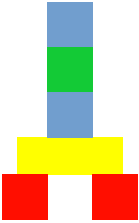
\includegraphics[scale=0.20]{figures/chapter2/task_goal.pdf}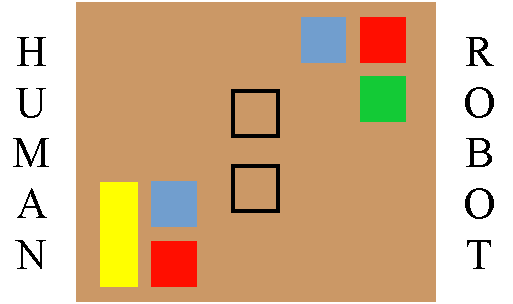
\includegraphics[scale=0.18]{figures/chapter2/task_setup_mini.pdf}}   
	\fancyhead[RO]{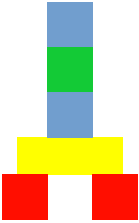
\includegraphics[scale=0.20]{figures/chapter2/task_goal.pdf}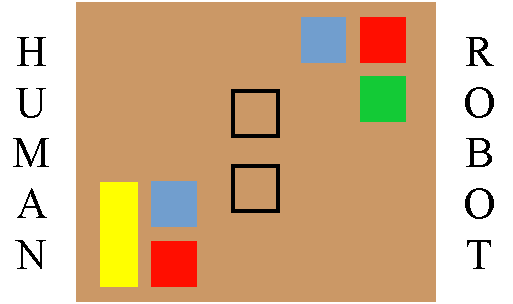
\includegraphics[scale=0.18]{figures/chapter2/task_setup_mini.pdf}\bfseries\thepage}  
	\fancyhead[RE]{\bfseries\nouppercase{\leftmark}}      % Chapter in the right on even pages
	\fancyhead[LO]{\bfseries\nouppercase{\rightmark}}     % Section in the left on odd pages
}%

\usepackage{pdfpages}
\usepackage{makecell}
\usepackage{pdflscape} 
\usepackage{mathtools}
\usepackage[section]{placeins}
\usepackage{afterpage}

%%%%%%%% my commands
\newcommand{\etal}{\textit{et al}.}
\newcommand{\ie}{\textit{i.e.}, }
\newcommand{\eg}{\textit{e.g.}, }
\newcommand{\fact}[3]{\mbox{\textit{#1}(#2, #3)}}
\newcommand{\circledtext}[1]{\raisebox{.5pt}{\textcircled{\raisebox{-.9pt} {#1}}}}
\newcommand{\sparql}{\textsc{SPARQL}}

\newcommand{\algConst}[1]{${\scriptscriptstyle #1}$}
\newcommand{\algNormTextSub}[2]{$\text{#1}_{#2}$}

\newcommand{\aslnumber}[1]{$#1$}
\newcommand{\aslstring}[1]{\textsf{#1}}
\newcommand{\aslvar}[1]{\textcolor{purple}{\textit{#1}}}
\newcommand{\asllabel}[1]{\textbf{#1}}
\newcommand{\annotation}[1]{{\footnotesize #1}}
\newcommand{\rulebody}[1]{\mbox{\hspace{.05\linewidth}}\begin{minipage}[t]{0.9\linewidth}#1.\end{minipage}}
\newcommand{\context}[1]{\begin{minipage}[t]{0.9\linewidth}#1\end{minipage}}
\newcommand{\planbody}[1]{\begin{minipage}[t]{0.9\linewidth}#1.\end{minipage}}
\newcommand{\Jason}[0]{\textbf{\textit{Jason}}}
\newcommand{\sn}{\mbox{\large\textbf{\texttt{\textasciitilde}}}}


\sloppy
\begin{document}
	\setcounter{chapter}{2} %% Numéro du chapitre précédent ;)
	\dominitoc
	\faketableofcontents
	\fi

\chapter{A robot evaluating its contribution to a human-robot joint action}\label{chap2:sec:qoi}
\minitoc

The work presented in this section has been excerpted from a paper published in the Journal of Social Robotics~\cite{mayima_2021_towards}.

\section{Introduction}

Robots dedicated to Human-Robot interactions are not just machines receiving commands and executing them. They should be decisional agents with high-level goals, taking decisions (potentially taking into account social norms), and acting and reacting to not only their actions but those of other agents. Cognitive and interactive robots are becoming more and more capable thanks to the use of human-aware models and algorithms~\cite{kruse2013,thomaz_2016_computational}, with roboticists endowing them with the ability to execute their share of the work while adapting to contingencies, particularly those caused by human's behaviors and decisions~\cite{hoffman_2007_fluency,cakmak_2017,lemaignan_2017_artificial}. The decision-making process is based on a range of knowledge about the environment, the interaction, the context... Nevertheless, curiously and interestingly, very little has been done to allow the robot, while performing its collaborative or assistive activity, to permanently evaluate if things are going well or not, as humans do. We name this ability ``the measure of the Quality of Interaction from the robot point of view''. We believe that enriching the robot knowledge with a good estimation about how the interaction is going, could enhance its decision-making process and thus, its social behaviour.

For example, if the robot detects that the \acrshort{qoi} starts to drop, it can take a decision based on this information and act to try to improve the interaction quality (\eg it can choose to change some modalities such as the language in which it communicates with the human, the volume of its speakers, or the parameters of its planners). On the contrary, when the \acrshort{qoi} is high, the robot can decide to just continue the interaction as planned. Then, endowed with a \acrshort{qoi} Evaluator, a robot becomes more adaptive and performs better. Also, a very poor performance all along a task could allow the robot to assess that the human is not really engaged in the interaction, or even is trying to play the robot. In such a situation, the robot might perhaps better disengage. 
Finally, from a methodological point of view, a robot deployed in the wild able to assess interactions, has an asset compared to others as it could reduce the investment in material and human resources to perform user studies. And, a developer might use the logs to improve their design. 

In this paper, we only focus on the Quality of Interaction evaluation process and not on how to use its result for decision making. Therefore,  we present in the sequel the methods and tools we developed, allowing the robot to evaluate in real-time the quality of the human-robot collaborative activity it is involved in. It is based on a set of metrics we have defined, focused on two concepts: the measure of human engagement and the measure of the effectiveness of collaborative tasks performance. However, this is by no means exhaustive, and other metrics and parameters could (and should) be added later. Our work can be seen as a toolbox among which it is possible to pick the desired metrics according to tasks or contexts. We propose a way to aggregate these metrics, producing the \acrshort{qoi}. The evaluation of the \acrshort{qoi} is performed at three different levels of abstraction: the interaction session level, the task level and the action level. In further work, this ability could provide additional information to the robot and open the possibility for reconsidering its behaviour in case it estimates that the quality of the interaction is degrading (\eg changing its plan or the way it is achieving it, informing the human or requesting a change in their behaviour, or even deciding to disengage).

The section is organized as follows. First, we briefly discuss related work and the main challenges. In section~\ref{chap2:sec:levels} we present the representation of human-robot collaborative activity which we use and its hierarchical  decomposition. Finally, in sections \ref{sec:eval} and \ref{sec:metrics}, we introduce our concept and proposed set of metrics to evaluate the Quality of Interaction. Example on a real task and proof-of-concept are presented in Chapter~\ref{chapter:chap3}.

\section{Related work}\label{sec:rel}

Inspired from the evaluation methods used in Human-Computer Interactions and User Experience fields, the field of Human-Robot Interaction (HRI) has elaborated its own methods to evaluate robotic systems when they interact with humans. There are various ways to evaluate a human-robot interaction from the human perspective. Bethel \textit{et al}.~\cite{bethel_2010_review} divided them into five categories: \begin{inlineEnumerate}
	\item self-assessments,\label{list:m_self}
	\item interviews,\label{list:m_inter}
	\item behavioral measures,\label{list:m_beha}
	\item psychophysiology measures, and\label{list:m_physio}
	\item task performance metrics\label{list:m_task}
\end{inlineEnumerate}. They reviewed metrics used for each of the categories. They can be grouped into two types: \ref{list:m_self} and \ref{list:m_inter} are subjective metrics and, \ref{list:m_beha}, \ref{list:m_physio} and \ref{list:m_task} are objective ones. Since our aim is to have a robot able to evaluate interactions by itself, human subjective metrics are not usable. Then we focused on the study of existing objective metrics meant to measure how the interaction goes. Steinfeld \textit{et al}.~\cite{steinfeld_2006_common} proposed a set of metrics to be used in a wide range of tasks whose goal is to assess the system performance by measuring the task effectiveness (\ie how well the task is completed) and the task efficiency (\ie the time required to complete a task). Their work is very thorough and inspiring but does not target the evaluation of the quality of an on-going interaction. 
Hoffman~\cite{hoffman2019} defined a type of quality of interaction, the \textit{fluency}, pointing out that the notion is not well defined and somewhat vague but can still be assessed and recognized when compared to non-fluent scenario. To measure it, they proposed a list of objective metrics, only based on duration measures, designed to be quite general: robot idle time, human idle time, concurrent activity (\ie active time of both the robot and the human), functional delay (\ie time difference between the end of one agent’s task and the beginning of the other agent’s task). It is an interesting way to measure the fluency and thus the quality of the human-robot interaction but it only applies to shared workspace tasks and is dedicated to an offline evaluation.

Systems targeting real-time measurements during human-robot interactions, with the purpose to ``close the loop'' and use the information for decision-making, have been developed. Tanevska \textit{et al}.~\cite{tanevska:hal-01615491} proposed a framework allowing the robot to perceive with face detection and evaluate in real-time the affective state (\ie anger, happiness, sadness, surprise, etc) and the engagement state (\ie whether the person is interested or bored in the interaction) of the people it is interacting with. However, the human affective state measure might not be enough to assess an interaction or a task as an affective state is actually a facial expression which can be misinterpreted (\eg a smile can be a sign of happiness or embarrassment) and which might be not visible when one of the agent performs an action and looks somewhere else. Moreover, as the notion of engagement is very task specific, it needs further exploration. Real-time engagement measurement has also been investigated by Anzalone \textit{et al}.~\cite{anzalone_2015_evaluating} using metrics such as gaze, head pose, body pose and response times. Their work is interesting and could be an element among others to assess the interaction quality but, it is dedicated to face-to-face interactions. 

Cameras are not the only sensor used to assess interactions on-the-fly, some use human physiological responses such as skin conductance and temperature, heart or brain signals. Itoh \textit{et al}.~\cite{itoh2006}, Bekele \textit{et al}.~\cite{bekele_2014} or Kulic \textit{et al}.~\cite{kulic2007} use them to detect human affective states such as anxiety or liking in real-time. However, physiological measures often imply a lot of sensors which can be invasive for the human. And, as explained by Kulic and Croft~\cite{kulic_2003_estimating}, physiological signals may be difficult to interpret and there is a large variability in physiological response from person to person. Thus, it can be difficult for a controller to determine which emotional state the subject is in, or whether the response was caused by an action of the system, or by an external stimulus. Moreover, we claim that the human affective state only is not enough to assess the quality of an interaction, a human could be satisfied with an interaction or a task result even though they were stressed during it.

Finally,  Bensch \textit{et al}.~\cite{bensch17} proposed a formal approach to compute interaction quality in real-time. Their work focused on how to combine metrics together which is in the same line as ours. However, they do not provide implementation examples, remaining at an abstract level.

In summary, while a substantial number of studies have been devoted to the evaluation of collaborative interactions for analysis purposes once the interaction is over, there is a lack of methods allowing the robot to evaluate in real-time the quality of the interaction based on multiple metrics and not only anxiety or engagement. We claim that such an ability is very important and should strongly influence the situation assessment as well as the decisional abilities of interactive and collaborative robots. 




\section{The Quality of Interaction (QoI)}\label{sec:eval}

We believe the real-time assessment of the \acrshort{qoi} with a human partner (\ie what the robot ``thinks'' about how the interaction is going) is a new knowledge that could enhance the robot decision-making process. We define the Quality of Interaction as a measure that indicates how good is the interaction during human-robot collaborative activities. It is computed in real-time based on a set of metrics, at three different levels: the interaction session level, the tasks level and the actions level. The \acrshort{qoi} of a given level is computed from selected metrics but also from the \acrshort{qoi}s of the level below as shown in Fig.~\ref{fig:qoi_schema}.

\begin{figure}[!ht]
	\centering
	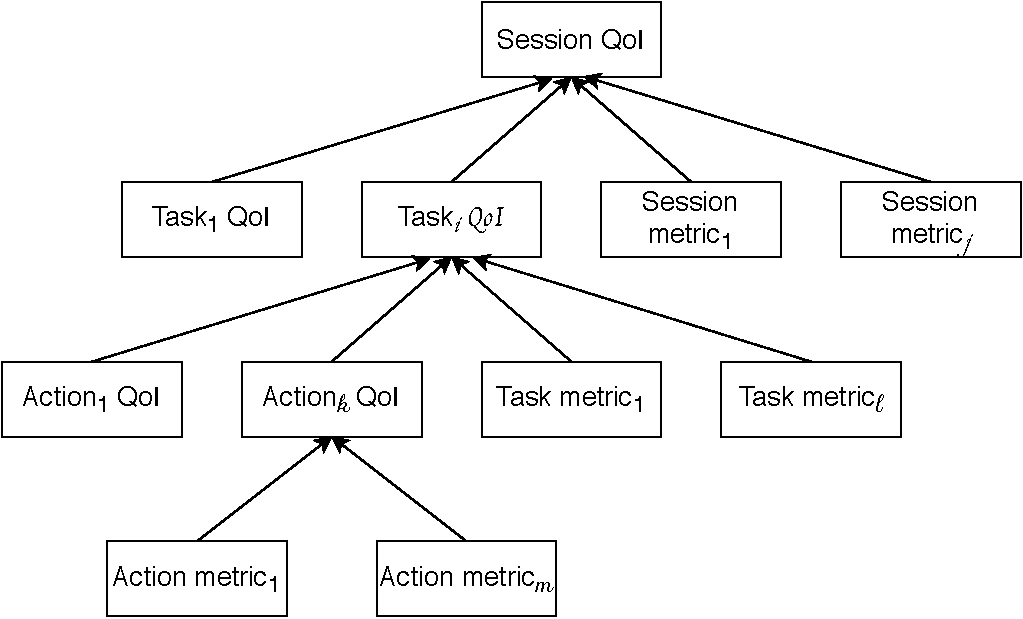
\includegraphics[width=\linewidth]{figures/chapter2/QoI_schema.pdf}
	\caption{Representation of the \acrshort{qoi} dependencies, with $i$ the number of performed tasks during the interaction session, $k$ the number of performed actions during the task $i$, $j$ the number of metrics to measure the interaction session \acrshort{qoi}, $l$ the number of metrics to measure the task $i$ \acrshort{qoi} and $m$ the number of metrics to measure the action $k$ \acrshort{qoi}.}
	\label{fig:qoi_schema}
\end{figure}

The \acrshort{qoi} of each level is computed as a score between [($1$) for a good quality] and [($-1$) for a poor one]. Metrics used to compute the \acrshort{qoi} are divided in three categories: 
\begin{bulletList}
	\item $Mp \in [0,1]$ if it can only have a positive effect on the evaluation;
	\item $Mn \in [-1,0]$ if a metric can only have a negative effect on the evaluation;
	\item $M \in [-1,1]$ if a metric can have a positive or a negative effect.
\end{bulletList}

Defined by the designer according to the needs and context, a metric can belong to one category or another depending on the target application. When needed, metrics values are scaled with the equations presented in Appendix~\ref{annex:functions}.

The evaluation of the Quality of Interaction at the level $l \in \{session_f,task_j,action_k\}$ (with $f,j \text{ and }k$ respectively the identifiers of a given interaction session, task and action),  $QoI_l$, is computed with:

\begin{equation}\label{eq:qoi}
QoI_{l}= \frac{ \sum\limits_{i=0}^x W_i * M_i}{\sum\limits_{i=0}^x W_i} + A * \frac{ \sum\limits_{i=0}^y Wn_i * Mn_i  + \sum\limits_{i=0}^z Wp_i * Mp_i}{\sum\limits_{i=0}^y Wn_i+\sum\limits_{i=0}^z Wp_i} 
\end{equation}


with $W_i, Wp_i,Wn_i$ respectively the corresponding designer-set weights of $M_i, Mp_i, Mn_i$, $A$ the designer-set weight of the right part of the $+$ sign and $x$, $y$, $z$ respectively the number of the metrics $M_i, Mp_i, Mn_i$.

Equation~\ref{eq:qoi} aggregates the values of the metrics chosen to be indicators of the interaction level quality. As all metrics do not have the same importance in the measure of the \acrshort{qoi}, each of them is weighted. Values of these weights are empirically defined. There are two parts in the equation, the left part of the $+$ sign and the right part. The left part of the $+$ sign is a weighted mean of the third category of metrics, the $M$ metrics. The right part is a weighted mean of the metrics seen as bonus (\ie $Mp$ metrics) or penalty (\ie $Mn$ metrics). This latter part is weighted with $A$ -- whose value is also empirically\footnote{Values are empirically defined given intuition regarding the importance of a given metrics for a given task and a set of testing experiments} defined -- to be able to adjust its influence on the left part. In such a way, if there are no $Mn$ metrics to compensate for the $Mp$ metrics, it is possible to limit the positive influence of the $Mp$ metrics on the $M$ metrics with $A$. It is the same if there are no $Mp$ metrics, $A$ can compensate the impact of the $Mn$ metrics on the $M$ metrics. Even though $M, Mp, Mn \in [-1,1]$, the final result of $QoI_l$ might be less than $-1$ or greater than $1$ because of the addition of the $M$ with the $Mn$ and $Mp$. If it happens, $QoI_l$ minimal value is set to $-1$ and its maximal value is set to $1$.

\section{A set of metrics}\label{sec:metrics}

In this section, we present a few measures to assess the \acrshort{qoi} of an interaction session in Sect.~\ref{subsec:m_intersess}. Then, we present metrics for the different levels based on engagement in Sect.~\ref{subsec:m_engag} and effectiveness estimations during human-robot joint activities in Sect.~\ref{subsec:task_eff}. For example, if the human is engaged and if tasks are performed effectively, the \acrshort{qoi} will tend to be high and \textit{vice versa}. Both concepts are difficult to measure, so we do not exactly measure them but we compute their trends from the set of metrics presented in this section. This set is not exhaustive and will be extended in future work but it gave promising results as we show with our implementation in Chapter~\ref{chapter:chap3}. All metrics are meant to be used for online evaluations of interactions. They are summarized in Table~\ref{tab:theo_metrics}.

\begin{table*}[t]
	\centering
	\begin{tabular}{|c|p{0.5cm}|p{3cm}|p{3.5cm}|c||c|c|c|}
		\hline
		&  \multicolumn{2}{c|}{Metric names} & Measures & Illustration & Session & Task & Action \\
		\hline\hline
		\multirow{10}{*}{\rotatebox[origin=t]{90}{Effectiveness}} & \multirow{6}{*}
		{\rotatebox{90}{Progress towards goal}} & Distance-to-Goal  & Geometric distance & \parbox[c]{3.5cm}{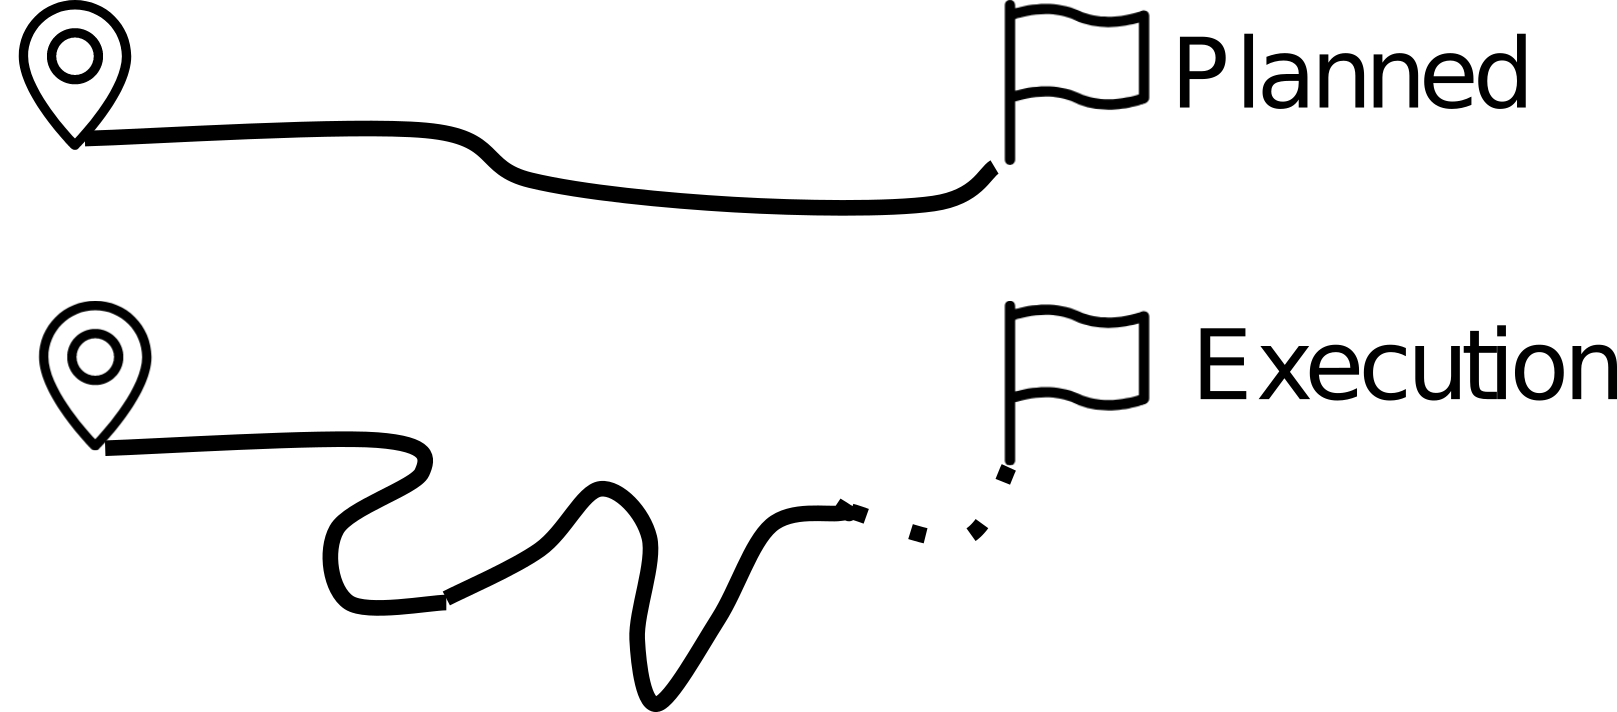
\includegraphics[width=3.5cm]{figures/chapter2/dtg.png}} & & x & x \\\cline{3-8}
		& & Time-to-Goal & Time & \parbox[c]{3.5cm}{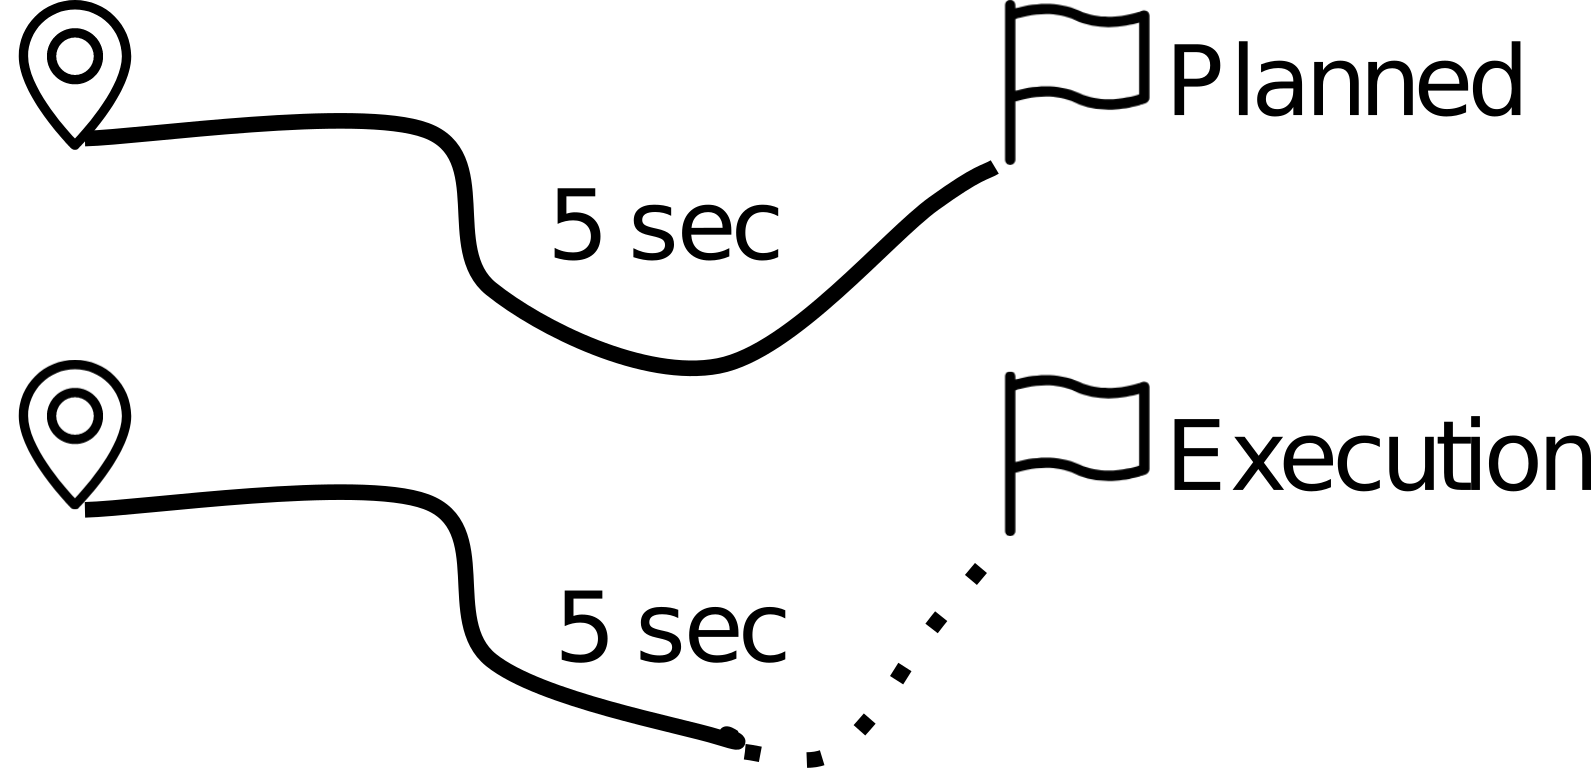
\includegraphics[width=3.5cm]{figures/chapter2/ttg.png}} & & x & x\\\cline{3-8}
		&  & Steps-to-Goal & Number of executed actions/substasks & \raisebox{-0.3cm}{\parbox[c][1.5cm]{3cm}{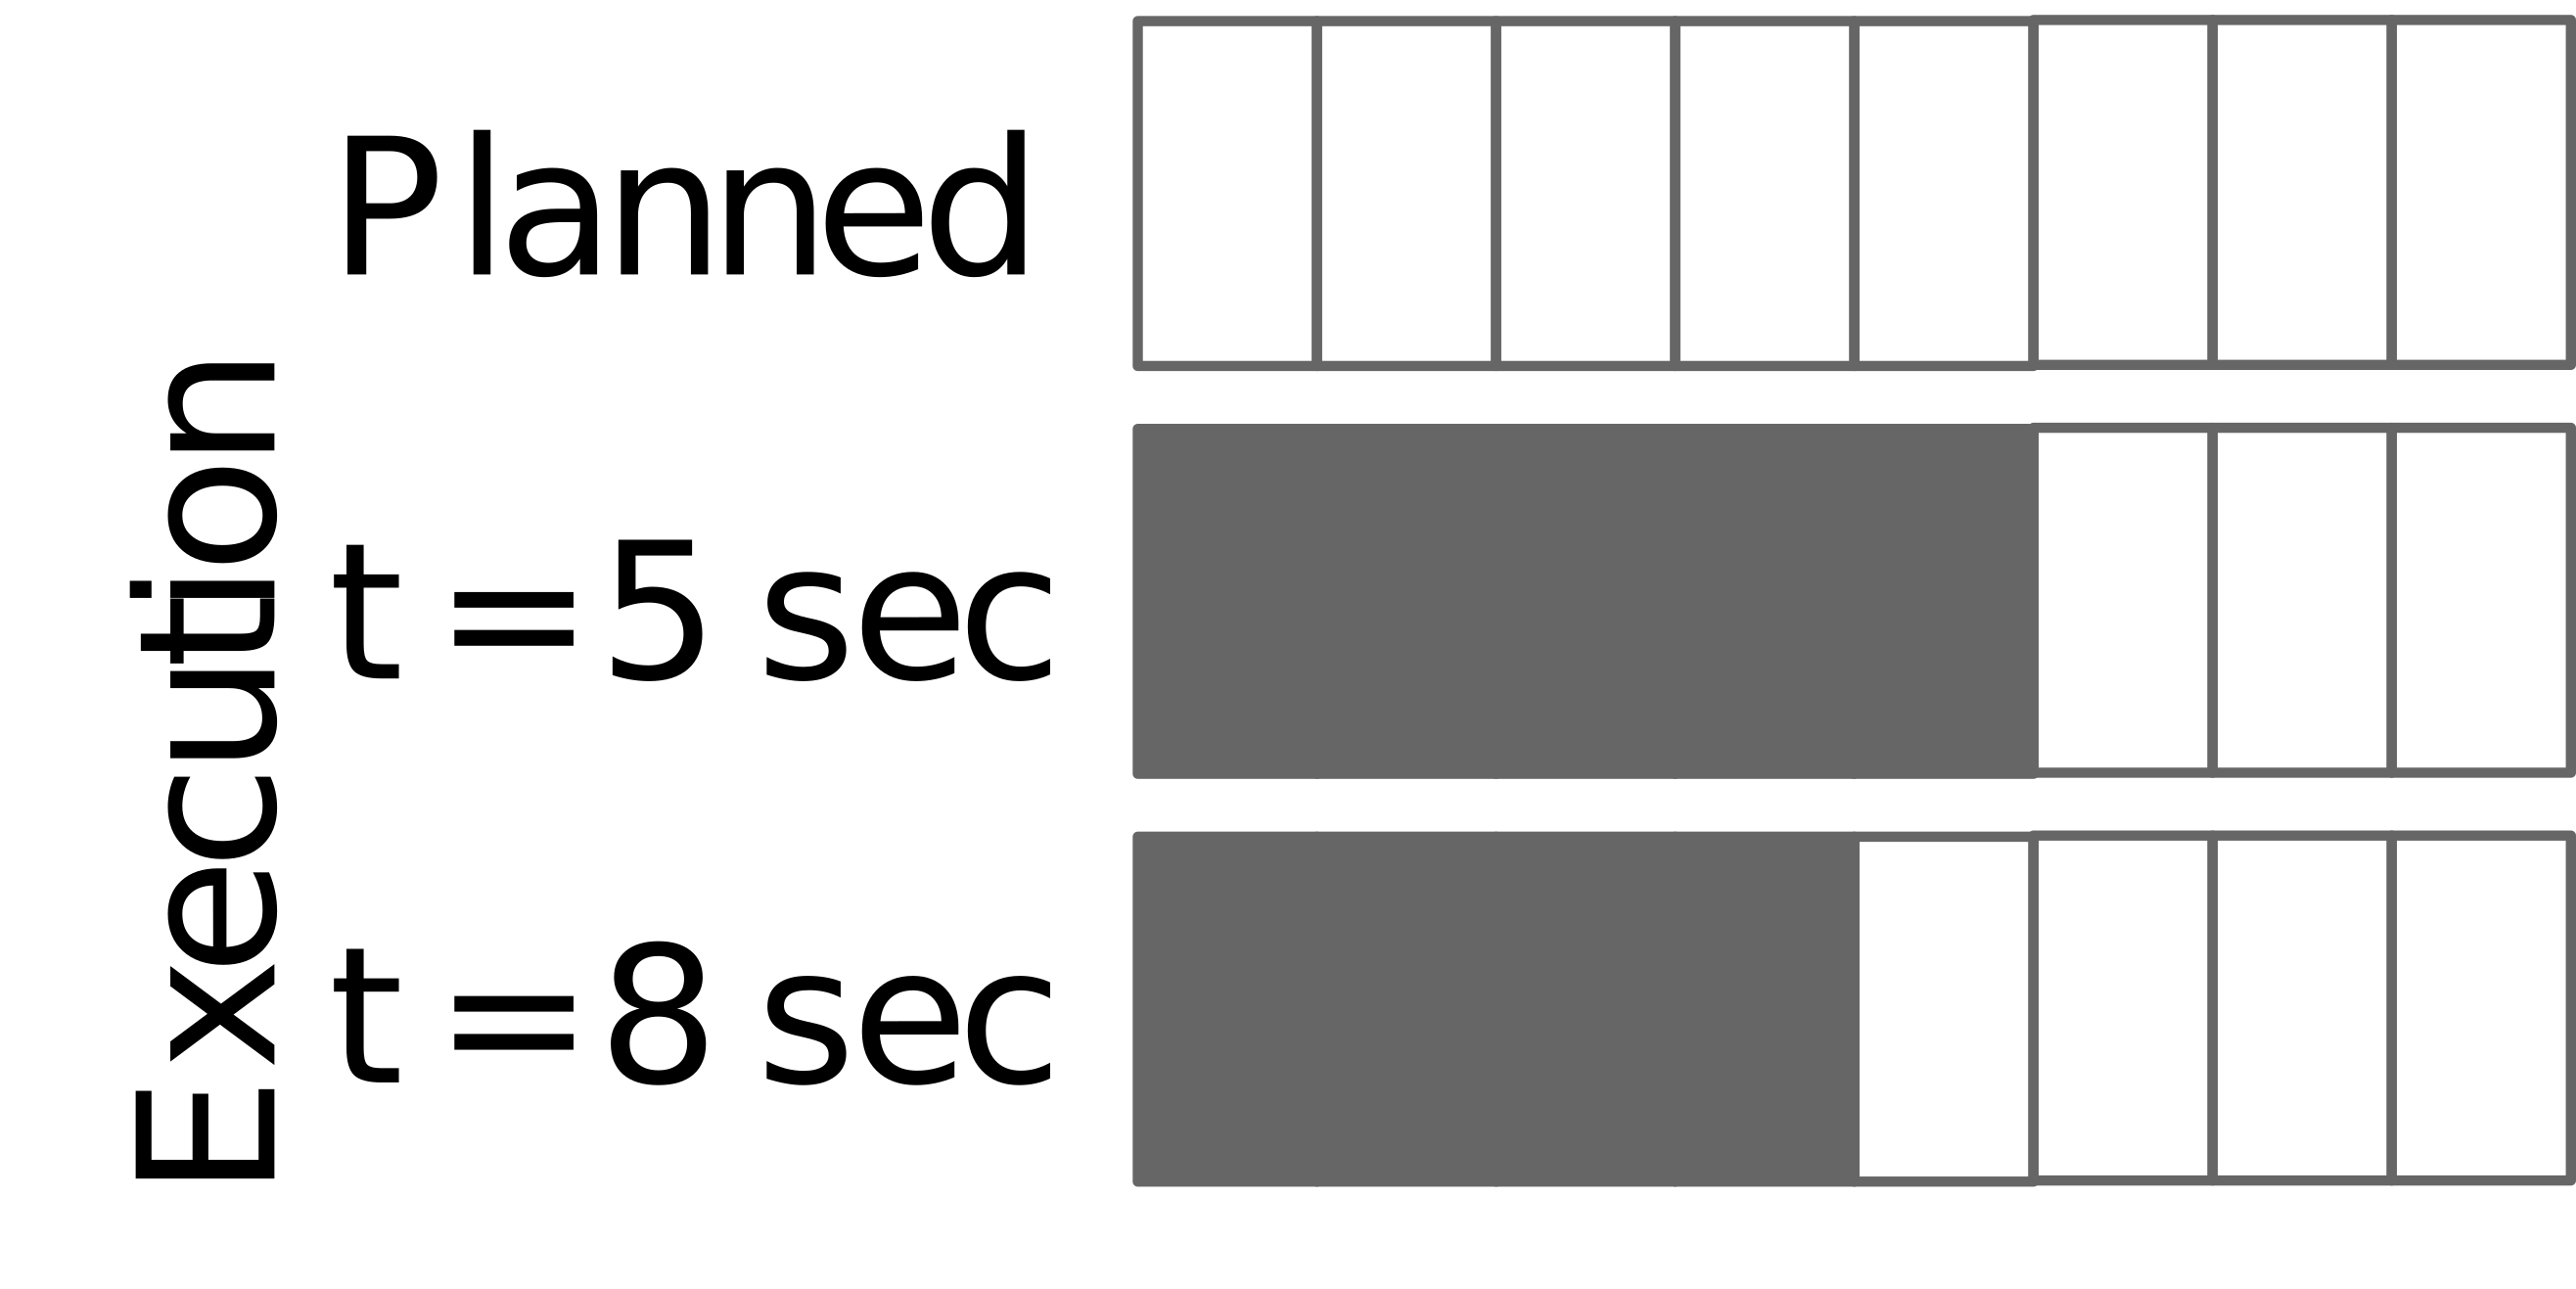
\includegraphics[width=3cm]{figures/chapter2/stg.png}}}&  & x &  \\\cline{2-8}
		&  \multicolumn{2}{p{3.5cm}|}{Deviation from standard duration} & Time & \parbox[c][1.2cm]{3.5cm}{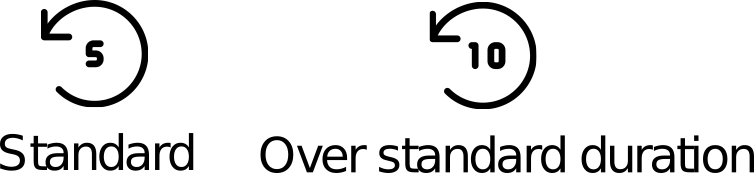
\includegraphics[width=3.5cm]{figures/chapter2/dd.png}}& & x & x \\\hline
		\multirow{5}{*}{\rotatebox[origin=c]{90}{Engagement}} 
		&  \multicolumn{2}{p{3.5cm}|}{Fulfilling robot expectations about social interaction} & \eg attention ratio, with-me-ness,... & \raisebox{-0.6cm}{
\includegraphics[width=3.5cm]{figures/chapter2/ar.png}}&x & x & x \\\cline{2-8}
		&  \multicolumn{2}{p{3.5cm}|}{Human contribution to the goal} & \eg number of repeated instructions, number of successful human actions,... & \raisebox{-0.8cm}{{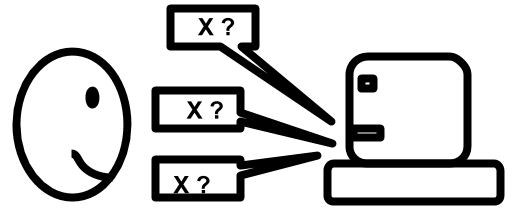
\includegraphics[width=2.4cm]{figures/chapter2/cg.png}}} & & x & x \\\hline
		% &  \multicolumn{2}{c|}{Interaction continuation} & \eg duration, number of tasks/actions, termination manner & x & x & \\\hline
	\end{tabular}
	\caption{The set of metrics presented in Section~\ref{sec:metrics}.}
	\label{tab:theo_metrics}
\end{table*}     


\subsection{Measures to assess the QoI at the interaction session level}\label{subsec:m_intersess}
According to the context, the duration of an interaction session can be an indicator of the human engagement. Indeed, a human leaving only a few seconds after the beginning of the interaction is probably less engaged than a human staying with the robot several minutes. Also depending on the context, the number of executed tasks is a measure which can be considered as interesting information with respect to the engagement of the human, as well as the ratio of successful tasks. The more the human executes successful tasks with the robot, the higher the session \acrshort{qoi} might be. Finally, it can be valuable to take into account how the session has been terminated in the evaluation of the quality of an interaction session. For instance, the fact that the human leaves abruptly in the middle of a task, during an idle time or a conversation without saying goodbye, or only at an appropriate time saying farewell to the robot is significant in terms of social interaction quality.

\subsection{Metrics related to human engagement}\label{subsec:m_engag}
Michael \textit{et al.}~\cite{michael2016} stated that commitments\footnote{In the robotic domain, it is the word ``engagement'' and not ``commitment'' which is often used, unlike in the psychological and philosophical fields.} facilitate ``the planning and coordination of joint actions involving multiple agents. Moreover, commitment also facilitates cooperation by making individuals willing to contribute to joint actions to which they would not be willing to contribute if they, and others, were not committed to doing so''. As it is an important element of the joint action, we want to provide the robot with a way to estimate the engagement of its partner during an interaction. 

Metrics allowing to state if an agent is engaged or not in an interaction are often specific to the type of interaction. For example, Fan \textit{et al.}~\cite{fan2017} implemented their measure of the human engagement as a kind of hysteresis: when the human gaze is on the robot, they are considered as engaged and when the human gaze is somewhere else during more than 3 consecutive seconds, they are considered as not-engaged. 

In the same vein, we think that the measure of the engagement for a collaborative activity can be divided in 2 types of metrics, summed up in Table~\ref{tab:theo_metrics}: the Human contribution to the goal and Fulfilling robot expectations about social interaction.

We define in this section examples of metrics of each types which can be used to estimate the level of engagement of the human partner. 

\paragraph{Human contribution to the goal}\label{subsubsec:h_contrib}

A good and very promising indicator could be the ability from the robot to evaluate how well the human actions help to the goal progression. We call this indicator \textit{Human contribution to the goal}. To the best of our knowledge, there is no general method to estimate it. 

As a first version of the \textit{Human contribution to the goal}, we chose to measure it through the number of times the robot has to repeat an instruction or a question before the human performs correctly, when it expects the human to answer or to perform the action. As, if it needs to repeat, it means that the human is not correctly contributing to the goal, intentionally or not, as they are not performing their part of the HR action as they should. The more the robot needs to repeat because of the human's bad performance, the less they are contributing to the goal, the more the action \acrshort{qoi} should decrease. 

\paragraph{Fulfilling robot expectations about social interaction}\label{subsubsec:r_exp}
During a social interaction, agents are expected to behave in a certain way and so the robot has expectations about the human. Then, the robot can monitor the human behavior to check if they are acting as they are expected to. For example, most of the time, when the robot speaks to the human, it will expect them to look at it and so it can monitor if it is the case or not as implemented by Fan \textit{et al.}~\cite{fan2017}. Quite similarly, Lemaignan \textit{et al.}~\cite{lemaignan2016} developed a way to measure if the human is \textit{with} the robot during their interaction, based on attention assessment, by computing if the human is looking at the desired attentional target or not. This latter metric will be integrated to our framework in future work.

As the works of Lemaignan \textit{et al.} and Fan \textit{et al.}, we estimate the \textit{Fulfilling robot expectations about social interaction} with the human head orientation, in the context of our implementation described in Chapter~\ref{chapter:chap3}. We compute an attention ratio \ie the time during which the human is attentive to the robot (\ie staying close enough and looking at it) when it speaks compared to the total time of the speech:

\begin{equation}\label{eq:attention_r}
Ar = \frac{duration_{isAttentiveTo(robot)=true}}{duration_{robot\_speaks}}
\end{equation}

\paragraph{Metrics related to effectiveness}\label{subsec:task_eff}
One can elaborate metrics to measure how well a task or an action is achieved. As discussed by Olsen and Goodrich~\cite{olsen_2003_metrics}, there are a variety of metrics such as time-based metrics which reward the speed of performance or the response times; error metrics which are based on counting retrials, failures, or mistakes; coverage metrics which measure to what extent a goal is achieved, as well as other possible metrics. We use some of them such as counting retrials, however these metrics alone were not enough for our example task as we are in an HRI context.

One can measure for different kinds of tasks, the ratio of successful\footnote{Obviously, the success is context and task dependent and should be defined according to the needs} executions to the total number of executions (\eg $R=\dfrac{Succ}{Exec}$) or the deviation from the initial plan (distance, cost, trajectory, etc). 

We define four metrics, summed up in Table~\ref{tab:theo_metrics}, allowing to measure the current task and action effectiveness. Three of them are means to measure how the progress towards the goal of a task or an action varies. Indeed, they are good indicators for the interaction quality as, when executing a task or an action, if the agents are not getting closer from the goal or even diverged from it, it means that something goes wrong. There are three different metrics because the one to use depends on the type of task or action. The fourth metric allows to compare the current execution duration to the standard execution duration of the task or action, based on durations measured during previous executions.

\paragraph{Metrics to assess the progress towards the goal}

We defined three different metrics to assess the progress towards the goal. The first one allows to assess the progress towards the goal of geometric-based actions. The second estimates the progress by using the remaining time to reach the goal. Finally, the last one measures the number of remaining steps (actions or substasks) before achieving the goal of a task.

\subparagraph{Distance-to-Goal}\label{para:dtg_gd} 
When an agent is performing a geometric-based action such as a movement, observing if the agent is getting closer to the target position over time provides a useful information about how well the action is going. Therefore, we introduce the \textit{Distance-to-Goal} $\Delta DtG$ metric: 
\begin{equation}\label{eq:dtgg}
\left\{
\begin{array}{ll}
\Delta DtG(t=0) = 0\\
\begin{aligned}
\Delta DtG(t) &= \max(0,\Delta DtG(t-1) - 1)  \\&\text{if } path\_length(t) <  path\_length(t-1) \\

\end{aligned}\\
\Delta DtG(t)= \Delta DtG(t-1) + 1, \text{otherwise.}

\end{array}
\right.
\end{equation}
with $path\_length(t)$ the length of the path leading the goal at time $t$ (\eg which can be given by a reactive motion planner~\cite{khamb2019}). The metric lower bound is 0. If at time $t$ the agent is closer to its final position than at $t-1$, \ie progressing towards their goal, the metric is set to decrease or to remain equal to 0. Now, if the agent has not moved or is even further, the metric increases. The closer the metric value is to 0, the better it is, as it means the distance to the goal has decreased over time. We chose to not directly compute the difference between  $path\_length(t)$ and  $path\_length(t-1)$ as the results would be very different whether it is an action implying a long path or a short path. 

\subparagraph{Time-to-Goal}\label{para:dtg_t}
This measure is intended to estimate the progress of a given task or action towards its goal based on the estimation of the remaining time to reach it. It compares the current estimated time to goal with the initial estimated time to goal taking into account the current task duration. As so, it is possible to measure the variation compared to the initial plan. We define the \textit{Time-to-Goal} $\Delta TtG$ as:
\begin{equation}\label{eq:ttg}
\Delta TtG(t) = \max(0, e(t)  + TtG(t) - TtG(T_0))
\end{equation}
with $e(t) = t - T_0$ the task execution duration (time elapsed since the beginning of the task), $TtG(t)$ the current time to the goal, and $TtG(T_0)$ the initial planned time to goal. In our work, $TtG(t)$ and $TtG(T_0)$ are provided by a reactive motion planner~\cite{khamb2019} because we used the metric for navigation but it could be provided by other kind of planners. 

\begin{figure}[!htb]
	\centering
	% Maximum length
	\subfloat[Plot of $\phi(t)_{X}$ of the subtask $X$ lasting 60 seconds, with $SD_{X}=10 sec$, $V_{X}=0.5$ and $\alpha=1$]{\label{fig:oteX}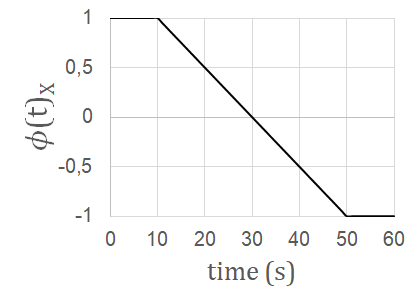
\includegraphics[width=0.49\linewidth]{figures/chapter2/oteX_2.png}}\hfill
	\subfloat[Plot of $\phi(t)_{Y}$ of the subtask $Y$ lasting 15 seconds, with $SD_{Y}=5 sec$, $V_{Y}=1$ and $\alpha=0.5$]{\label{fig:oteY}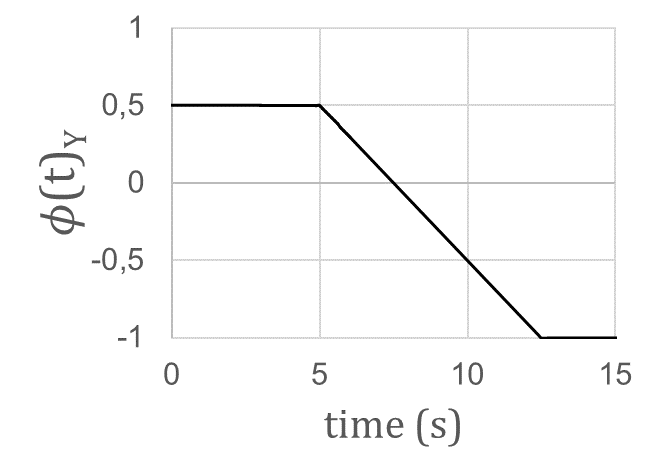
\includegraphics[width=0.49\linewidth]{figures/chapter2/oteY_2.png}}\hfill
	\subfloat[Plot of $\Phi(t)_{Ta}$ for a task composed of a sequence of three subtasks $X, Y, Z$: the duration of $X$ exceeded $SD_X=10 s$ and reached $20 s$, the duration of $Y$ exceeded $SD_Y= 5s$ and reached $10 s$, finally the duration of $Z$ was less than $SD_Z=10s$]{\label{fig:ote2}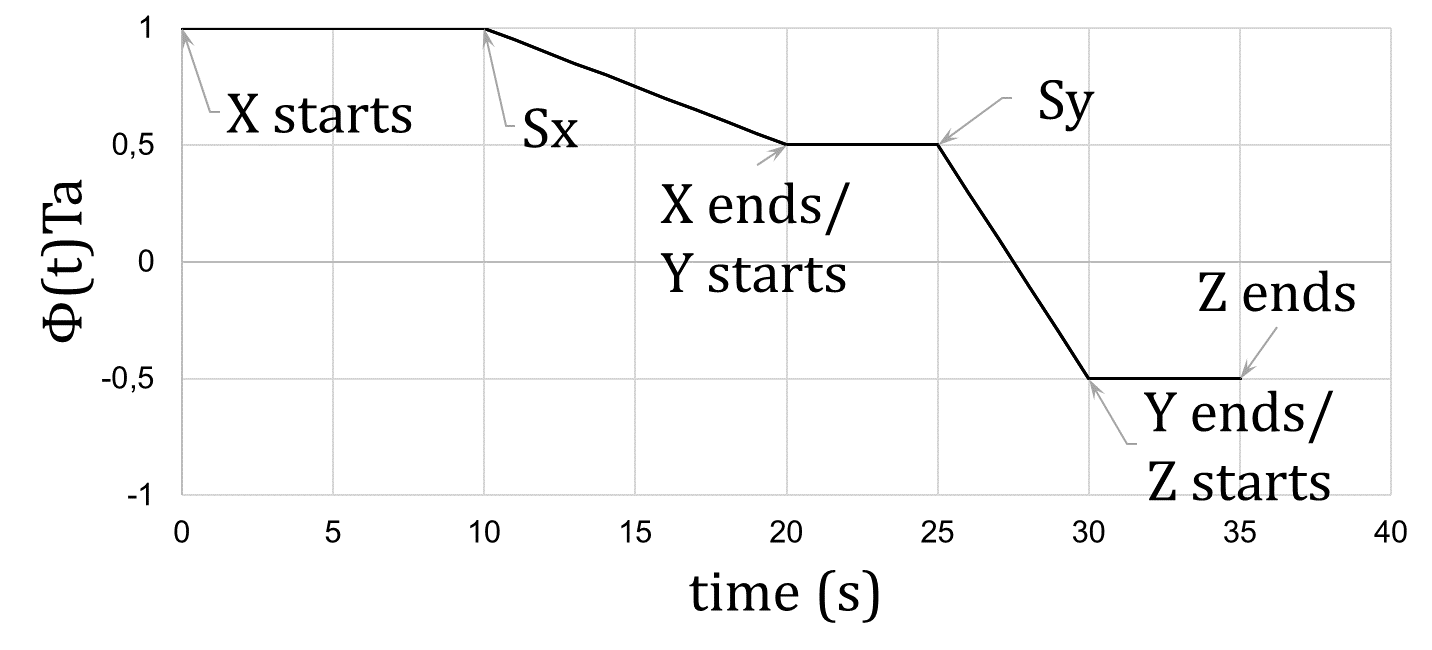
\includegraphics[width=0.7\linewidth]{figures/chapter2/ote.png}}\hfill
	\caption{Examples of plots of the $\phi$ and $\Phi$ functions}
	\label{fig:ote}
\end{figure}

\subparagraph{Steps-to-Goal}
One way to estimate the remaining distance to the goal for a task is to count the number of remaining substasks or actions (depending on the relevant scale) to perform. In addition, one can add a factor which estimates the weight (or effort needed) of each action or subtask. These weights can be determined by the designer, provided by the planner, etc. 
Then, the \textit{Steps-to-Goal} $\mathcal{D}$  of a task can be computed as time $t$:
\begin{equation}\label{eq:edtgs}
\mathcal{D}(t) = \dfrac{\sum\limits_{i=1}^c \mathcal{W}_i}{\sum\limits_{i=1}^n \mathcal{W}_i}
\end{equation}
with $\mathcal{W}_i$ the weight of a subtask/action $i$, $c$ the number of completed subtasks/actions and $n$ the total number of planned subtasks/actions.

\paragraph{Deviation from standard duration}\label{subsubsec:ote}
We introduce here a metric to measure the deviation from standard execution duration, the \textit{Deviation from standard duration} $\phi$ for subtasks/actions and the \textit{Deviation from standard duration} $\Phi$ for a whole task. This measure is intended to represent the degradation of the quality of execution of an HR task when its duration exceeds a certain time. 

To each subtask/action $a_i$, we associate two attributes whose values are defined by the designer: a soft deadline $SD_i$ and a decreasing quality  speed $V_i$. 
If, at time $t$, the execution duration  $e(t) = t - T_0$ of a substask or action $a_i$ which has started at $T_0$ exceeds $SD_i$, the quality will decrease over time at speed $V_i$: 
\begin{equation}\label{eq:ote}
\phi(t)_i=\max\left( V_i*\frac{-\max(e(t)-SD_i,0)}{SD_i}+\alpha,-1\right)
\end{equation}
where $\alpha$ is the value initial value and the upper bound (as at $t=0$, $\max(e(t)-SD_i,0)=0$) of $\phi_i$, when the subtask/action $a_i$ starts.

Then, we define a metric $\Phi$ for a task. It is an aggregation of the $\phi_i$ computed for each performed subtask/action $a_i$ of the task. At any moment, $\Phi$ can be seen as a memory of the previous steps, so the initial value $\alpha$ of $a_i$ is equal to the final value of $\phi_{i-1}$ of the previous subtask/action $a_{i-1}$, $\alpha=\phi(T_{final})_{i-1}$.


We can notice that it is not possible for this metric to increase over time since it memorizes the values of the previous actions. However, the total computed \acrshort{qoi} can get higher thanks to the other metrics. Moreover, $\phi$ can be used independently of $\Phi$. In such a case, the initial of value $\alpha$ of $\phi$ can be set to 1. 

Three examples are given in Fig.~\ref{fig:ote}. Fig.~\ref{fig:oteX}~and~\ref{fig:oteY} represent $\phi(t)_{X}$ and $\phi(t)_{Y}$ for two independent subtasks $X$ and $Y$. Fig.~\ref{fig:ote2} is a plot of $\Phi(t)_{Ta}$ for the task $Ta$ composed of the subtasks $X, Y, Z$ with $SD_X=10 s$, $V_X=0.5$, $SD_Y=5 s$, $V_Y=1$, $SD_Z=10 s$ and $V_Z=1$.

\section{Conclusion}\todo{change according to how we'll modify the plan}
In the last section, we have described a novel concept, the evaluation of the \acrfull{qoi}. This concept will be demonstrated in Section~\ref{sec:qoi_integration}, in the context of the direction-giving task presented in Chapter~\ref{chapter:chap3}.

\ifdefined\included
\else
\bibliographystyle{acm}
\bibliography{These}
\end{document}
\fi
